\documentclass[10pt]{book}
\usepackage[inner=0.6in,outer=0.6in,top=0.7in,bottom=0.7in,a5paper]{geometry}
\usepackage{lingmacros}
\usepackage{tree-dvips}
\usepackage[dvipsnames]{xcolor}
\usepackage{tabto}
\usepackage{titlesec}
\usepackage{adjustbox}
\usepackage{etoolbox}
\usepackage{hyperref}
\usepackage{graphicx}
\usepackage{longtable}
\usepackage{multicol}
\usepackage{pdfpages}
\usepackage{fancyhdr}
\usepackage{parskip} 
\usepackage{tikz}
\usetikzlibrary{shadows}
\usetikzlibrary{backgrounds}
\usetikzlibrary{calc}
\usepackage{lipsum}% just to automatically generate text
%\usepackage{avant}
%\renewcommand*\familydefault{\sfdefault} %% Only if the base font of the document is to be sans serif
%\usepackage[T1]{fontenc}

%\usepackage{algolrevived}
%\usepackage{caladea}
%\usepackage{fontspec}
%\usepackage{utopia}
%\usepackage{tgpagella}
\usepackage{charter}

\title{DARIC}
\author{Daryl Dudey}
\date{February 2022}

\fancyhf{} % clear all header and footers
\renewcommand{\headrulewidth}{0pt} % remove the header rule
\fancyfoot[LE,RO]{\thepage} % Left side on Even pages; Right side on Odd pages
\pagestyle{fancy}
\fancypagestyle{plain}{%
  \fancyhf{}%
  \renewcommand{\headrulewidth}{0pt}%
  \fancyhf[lef,rof]{\thepage}%
}

\hypersetup{%
    pdfborder = {0 0 0}
}

\pagestyle{fancy}

\titleformat{\chapter}[display]   
{\normalfont\huge\bfseries}{\chaptertitlename\ \thechapter}{20pt}{\Huge}   
\titlespacing*{\chapter}{0pt}{-50pt}{40pt}

\setlength{\parindent}{0pt}
\setlength{\parskip}{0.35cm plus4mm minus3mm}

\definecolor{vlightgray}{gray}{0.9}
\definecolor{vvlightgray}{gray}{0.975}

\newcommand{\CC}{C\nolinebreak\hspace{-.05em}\raisebox{.4ex}{\tiny\bf +}\nolinebreak\hspace{-.10em}\raisebox{.4ex}{\tiny\bf +}}
\def\CC{{C\nolinebreak[4]\hspace{-.05em}\raisebox{.4ex}{\tiny\bf ++}}}

\newcommand{\example}[1]{\par{\fcolorbox{white}{vlightgray}{\texttt{\parbox{11.5cm}{#1}}}}\vskip0.1cm}
\newcommand{\out}[1] {\par{\fcolorbox{black}{vvlightgray}{\texttt{\parbox{11.5cm}{#1}}}}\vskip0.1cm}
\newcommand{\DARIC}{DARIC}
\newcommand{\oldti}{\textsuperscript{\tiny{\textit{int}}}}
\newcommand{\oldtr}{\textsuperscript{\tiny{\textit{real}}}}
\newcommand{\ti}{\%}
\newcommand{\tr}{\#}
\newcommand{\ts}{\$}
\newcommand{\tri}{\textit{int}=}
\newcommand{\trr}{\textit{real}=}
\newcommand{\trs}{\textit{string}=}
\newcommand{\opo}{\textcolor{lightgray}{(}}
\newcommand{\opc}{\textcolor{lightgray}{)}}
\newcommand{\oti}[1]{\textcolor{gray}{[,{#1}\textit{\%}]}}
\newcommand{\otr}[1]{\textcolor{gray}{[,{#1}\textit{\#}]}}
\newcommand{\codec}[1]{\fcolorbox{white}{vlightgray}{\texttt{#1}}}
\newcommand{\aoc}{\textsuperscript{\small{*}}}
\newcommand{\aoct}[3]{\par{\textit{\texttt{#1}{ or }\texttt{#2}{ may be used instead of }\texttt{#3}.}}}
\newcommand{\lref}[8]{
		\subsection{#1}
			\par{#4}
			\par{
				\textbf{Syntax:}\\
				\texttt{\large{#8#1#5}}
			}
			\par{\ifstrempty{#6}{}{#6}}
			%\aoct{#2}{#3}{#1}
			\par{
				\textbf{Example:}\\
				\fcolorbox{white}{vlightgray}{\texttt{\parbox{11.5cm}{#7}}}
			}
			\vskip1.0cm
}
\newcommand{\lreftwo}[9]{
		\subsection{#1}
			\par{#4}
			\\
			\par{
				\textbf{Syntax:}\\
				\texttt{\large{#9#1#5}}\\
				\texttt{\large{#9#1#6}}\\
			}
			\par{\ifstrempty{#7}{}{#7}}
			\aoct{#2}{#3}{#1}
			\par{
				\textbf{Example:}\\
				\fcolorbox{white}{vlightgray}{\texttt{\parbox{11.5cm}{#8}}}
			}
			\vskip1.0cm
}
\newcommand{\lrefi}[8]{
		\subsection{#1}
			\par{#4}
			\par{
				\textbf{Syntax:}\\
				\texttt{\large{#1#5}}
			}
			\par{\ifstrempty{#6}{}{#6}}
			\aoct{#2}{#3}{#1}
			\par{
				\textbf{Example:}\\
				\fcolorbox{white}{vlightgray}{\texttt{#7}}
			}
			\vskip1.0cm
}

\newcommand*\keystroke[1]{%
  \begin{tikzpicture}[baseline=(key.base), very thin, line cap=round, black, rounded corners=0pt]%
    \node [draw, fill=white, fill opacity=1, rectangle, rounded corners=2pt, inner sep=2pt, minimum width=1.8em, font=\scriptsize\sffamily] (key) {#1\strut};

    \begin{scope}[on background layer]
      \draw [rounded corners=1pt, fill=white] ($ (key.north west) + (-2pt, 2pt) $) rectangle ($ (key.south east) + (2pt, -2pt) $);
      \fill [gray!60] ($ (key.south west) + (2pt, 0.1pt) $) -- ($ (key.south west) + (-1pt, -2pt) $)
                  -- ($ (key.south east) + (1pt, -2pt) $)  -- ($ (key.south east) + (-2pt, 0.1pt) $) -- cycle;
      \fill [gray!60] ($ (key.south east) + (-0.1pt, 2pt) $) -- ($ (key.south east) + (2pt, -1pt) $)
                  -- ($ (key.north east) + (2pt, 1pt) $)    -- ($ (key.north east) + (-0.1pt, -2pt) $) -- cycle;
    \end{scope}

    \draw ($ (key.north west) + (0.1pt, -2pt) $) -- ($ (key.north west) + (-2pt, 1pt) $);
    \draw ($ (key.north west) + (2pt, -0.1pt) $) -- ($ (key.north west) + (-1pt, 2pt) $);

    \draw ($ (key.north east) + (-0.1pt, -2pt) $) -- ($ (key.north east) + (2pt, 1pt) $);
    \draw ($ (key.north east) + (-2pt, -0.1pt) $) -- ($ (key.north east) + (1pt, 2pt) $);

    \draw ($ (key.south west) + (0.1pt, 2pt) $) -- ($ (key.south west) + (-2pt, -1pt) $);
    \draw ($ (key.south west) + (2pt, 0.1pt) $) -- ($ (key.south west) + (-1pt, -2pt) $);

    \draw ($ (key.south east) + (-0.1pt, 2pt) $) -- ($ (key.south east) + (2pt, -1pt) $);
    \draw ($ (key.south east) + (-2pt, 0.1pt) $) -- ($ (key.south east) + (1pt, -2pt) $);
  \end{tikzpicture}%
}

\newcommand*\keystrokew[1]{%
  \begin{tikzpicture}[baseline=(key.base), very thin, line cap=round, black, rounded corners=0pt]%
    \node [draw, fill=white, fill opacity=1, rectangle, rounded corners=2pt, inner sep=2pt, minimum width=3.75em, font=\scriptsize\sffamily] (key) {#1\strut};

    \begin{scope}[on background layer]
      \draw [rounded corners=1pt, fill=white] ($ (key.north west) + (-2pt, 2pt) $) rectangle ($ (key.south east) + (2pt, -2pt) $);
      \fill [gray!60] ($ (key.south west) + (2pt, 0.1pt) $) -- ($ (key.south west) + (-1pt, -2pt) $)
                  -- ($ (key.south east) + (1pt, -2pt) $)  -- ($ (key.south east) + (-2pt, 0.1pt) $) -- cycle;
      \fill [gray!60] ($ (key.south east) + (-0.1pt, 2pt) $) -- ($ (key.south east) + (2pt, -1pt) $)
                  -- ($ (key.north east) + (2pt, 1pt) $)    -- ($ (key.north east) + (-0.1pt, -2pt) $) -- cycle;
    \end{scope}

    \draw ($ (key.north west) + (0.1pt, -2pt) $) -- ($ (key.north west) + (-2pt, 1pt) $);
    \draw ($ (key.north west) + (2pt, -0.1pt) $) -- ($ (key.north west) + (-1pt, 2pt) $);

    \draw ($ (key.north east) + (-0.1pt, -2pt) $) -- ($ (key.north east) + (2pt, 1pt) $);
    \draw ($ (key.north east) + (-2pt, -0.1pt) $) -- ($ (key.north east) + (1pt, 2pt) $);

    \draw ($ (key.south west) + (0.1pt, 2pt) $) -- ($ (key.south west) + (-2pt, -1pt) $);
    \draw ($ (key.south west) + (2pt, 0.1pt) $) -- ($ (key.south west) + (-1pt, -2pt) $);

    \draw ($ (key.south east) + (-0.1pt, 2pt) $) -- ($ (key.south east) + (2pt, -1pt) $);
    \draw ($ (key.south east) + (-2pt, 0.1pt) $) -- ($ (key.south east) + (1pt, -2pt) $);
  \end{tikzpicture}%
}

\makeatletter
\newcommand\ackname{Acknowledgements}
  \newenvironment{acknowledgements}{%
      \@beginparpenalty\@lowpenalty
      \begin{center}%
        \bfseries \ackname
      \end{center}}%

\begin{document}

\begin{titlepage}
    \centering
	
\includegraphics[width=8cm]{_Logo.png}\\
    \vskip1cm
	\setlength{\fboxrule}{1pt}
	\fbox{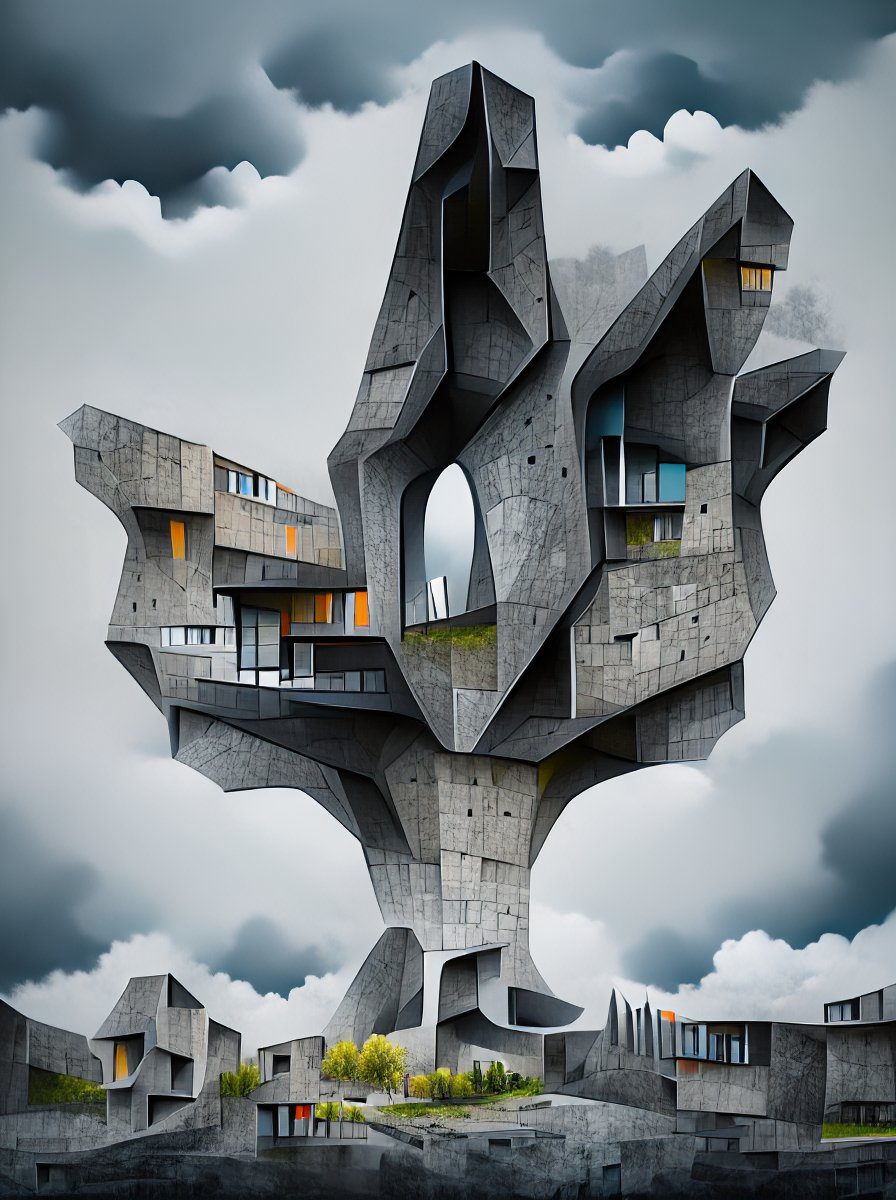
\includegraphics[height=11cm]{DARICFrontCover.jpeg}}
    \vskip1cm
    \huge{Daryl Dudey}
    \vskip0.25cm
    \normalsize{\emph{The creator of \DARIC{} and OS/D}}
\end{titlepage}
\begin{acknowledgements}
\par{My wife for not murdering me while writing the book. I'd disappear into my shed writing until late at night and she only occasionally complained.}
\par{Cover art printed with permission of the Unlimited Dream Co.}
\begin{center}
\emph{\url{https://unltddream.co}}
\end{center}
\par{I want to thank x, y z for testing \DARIC{}.}
\end{acknowledgements}

\tableofcontents

\chapter{Introduction}
\section{What is \DARIC?}

\subsection{The microcomputer revolution}
\par{I'm old. Well, not really, but my kids certainly think so. I grew up in the 1980s during the microcomputer revolution. It started in the US, with Altair the 8800, but it wasn't until the trio of the Commodore PET 2001, Apple II and TRS-80 Model 1 that it really started to become mainstream.}
\par{During the first few years of the 1980s, the US started to turn towards non-microcomputers such as the IBM PC and later the Apple Macintosh. However, in Europe, and in particular the UK where I live microcomputers (or micros) were dominant. This may have been because of cost, but also because Europe didn't have the console revolution that the US and Japan had - so there was far more focus on microcomputers.}
\par{In fact, the number of microcomputers released in Europe during 1980s was incredible. Most flopped of course, but a few did well and competed fairly successfully with American and Japanese imports.}
\begin{center}
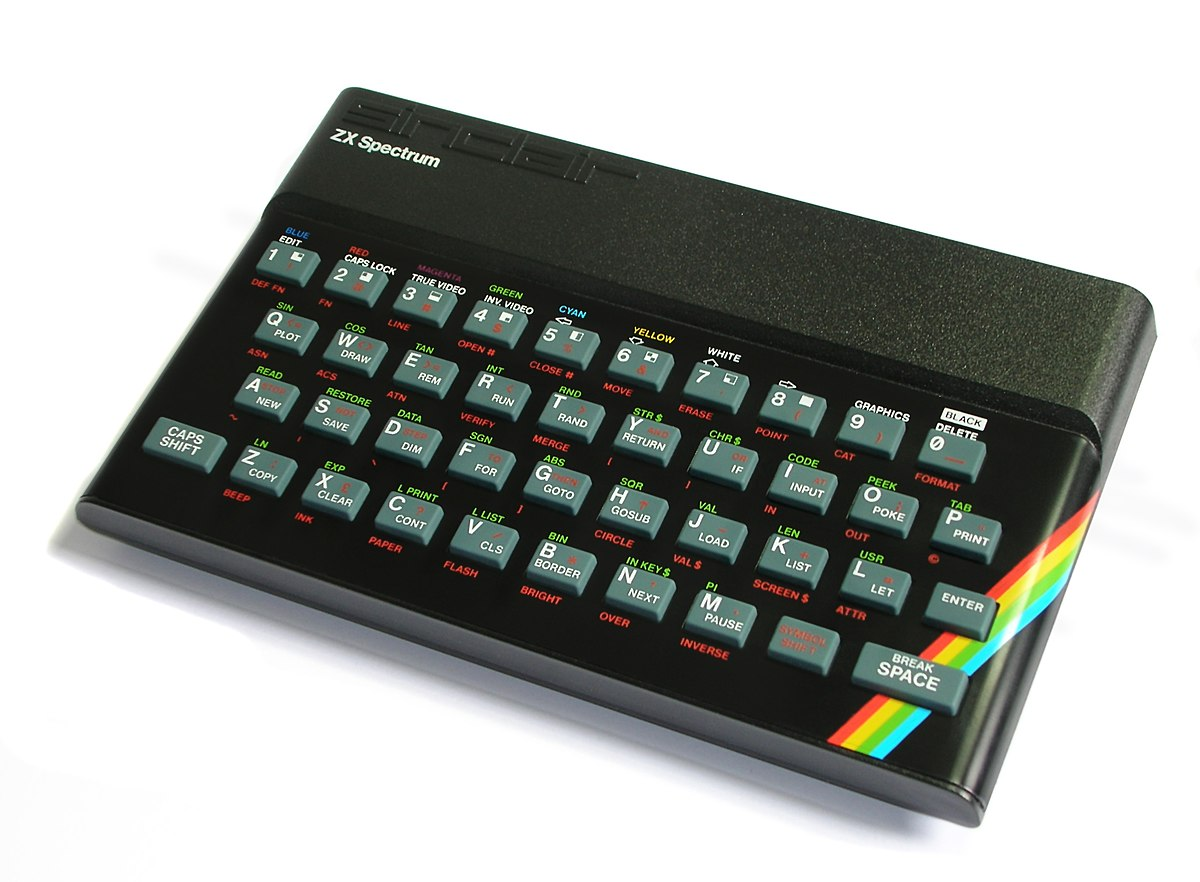
\includegraphics[height=3cm]{1200px-ZXSpectrum48k.jpg}\\
\scriptsize{\emph{The Sinclair ZX Spectrum.}}
\end{center}
\par{In school playgrounds, arguments ensued about whether the Sinclar ZX Spectrum was king because of the vast games library, or whether the Commodore 64 with it's superior graphics and sound was better. I owned a \emph{Speccie} so clearly it was the better machine! There were many other manufacturers: Amstrad, Acorn, Atari, Mattel, Oric etc.}
\par{This meant that there was an explosion of \emph{computer} games rather than \emph{video} games. There is some debate over the size of the ZX Spectrum games catalogue, but 23,000 seems an appropriate figure. Some were amazing, some were utterly awful.}
\subsection{Why is this relevant to \DARIC?}
\par{These early machines didn't boot from floppy disk drives, or hard drives. Floppy disk(ette) drives were expensive and relatively slow. As a result these machines booted from ROM. Unlike MS-DOS or CP/M, almost every machine booted to a BASIC prompt.}
\par{For many, this prompt was simply a way to \textbf{LOAD} or \textbf{CHAIN} their favourite game from cassette or (for the more \emph{middle class} kids) floppy disk.}
\par{However, for the more curious this flashing prompt held exciting potential. It wasn't uncommon for microcomputers to have a substantial manual in the box, which included a section on programming. After all, many parents were persuaded to buy these computers on the promise of helping their children learn - or conned in many cases!}

\subsection{The bedroom coder}
\par{This is where I started, and many others too. The potential felt limitless, there was BASIC, and for the more confident and capable - machine code. It was entirely possible, and indeed common for computer games to be written by a single person - often from home. They were termed 'bedroom coders'.}
\par{I wanted to create games and applications. With no formal education my programming style was haphazard at best, and the BASIC on my Sinclar ZX Spectrum didn't really allow particularly well structured code. I learned Z80 machine code, and was blown away by execution speed.}
\par{As I voraciously read programming books, it became obvious I was outgrowing the machine. Saving programs to tape was tedious, and frustrating. I walked to the local computer shop with my dad to look at Sinclair Microdrives. These were a much faster alternative to tape, and allowed more sensible management of files.}
\par{\emph{In an interesting twist, I ended up working for this shop for around a year at the start of my career!}}
\par{We went there to look at microdrives, and ended up walking out with an Acorn BBC Master 128 with twin 5$\frac{1}{4}$ inch floppy disk drives, and both of the reference manuals. This was obviously quite a surprise to twelve year old me! }
\begin{center}
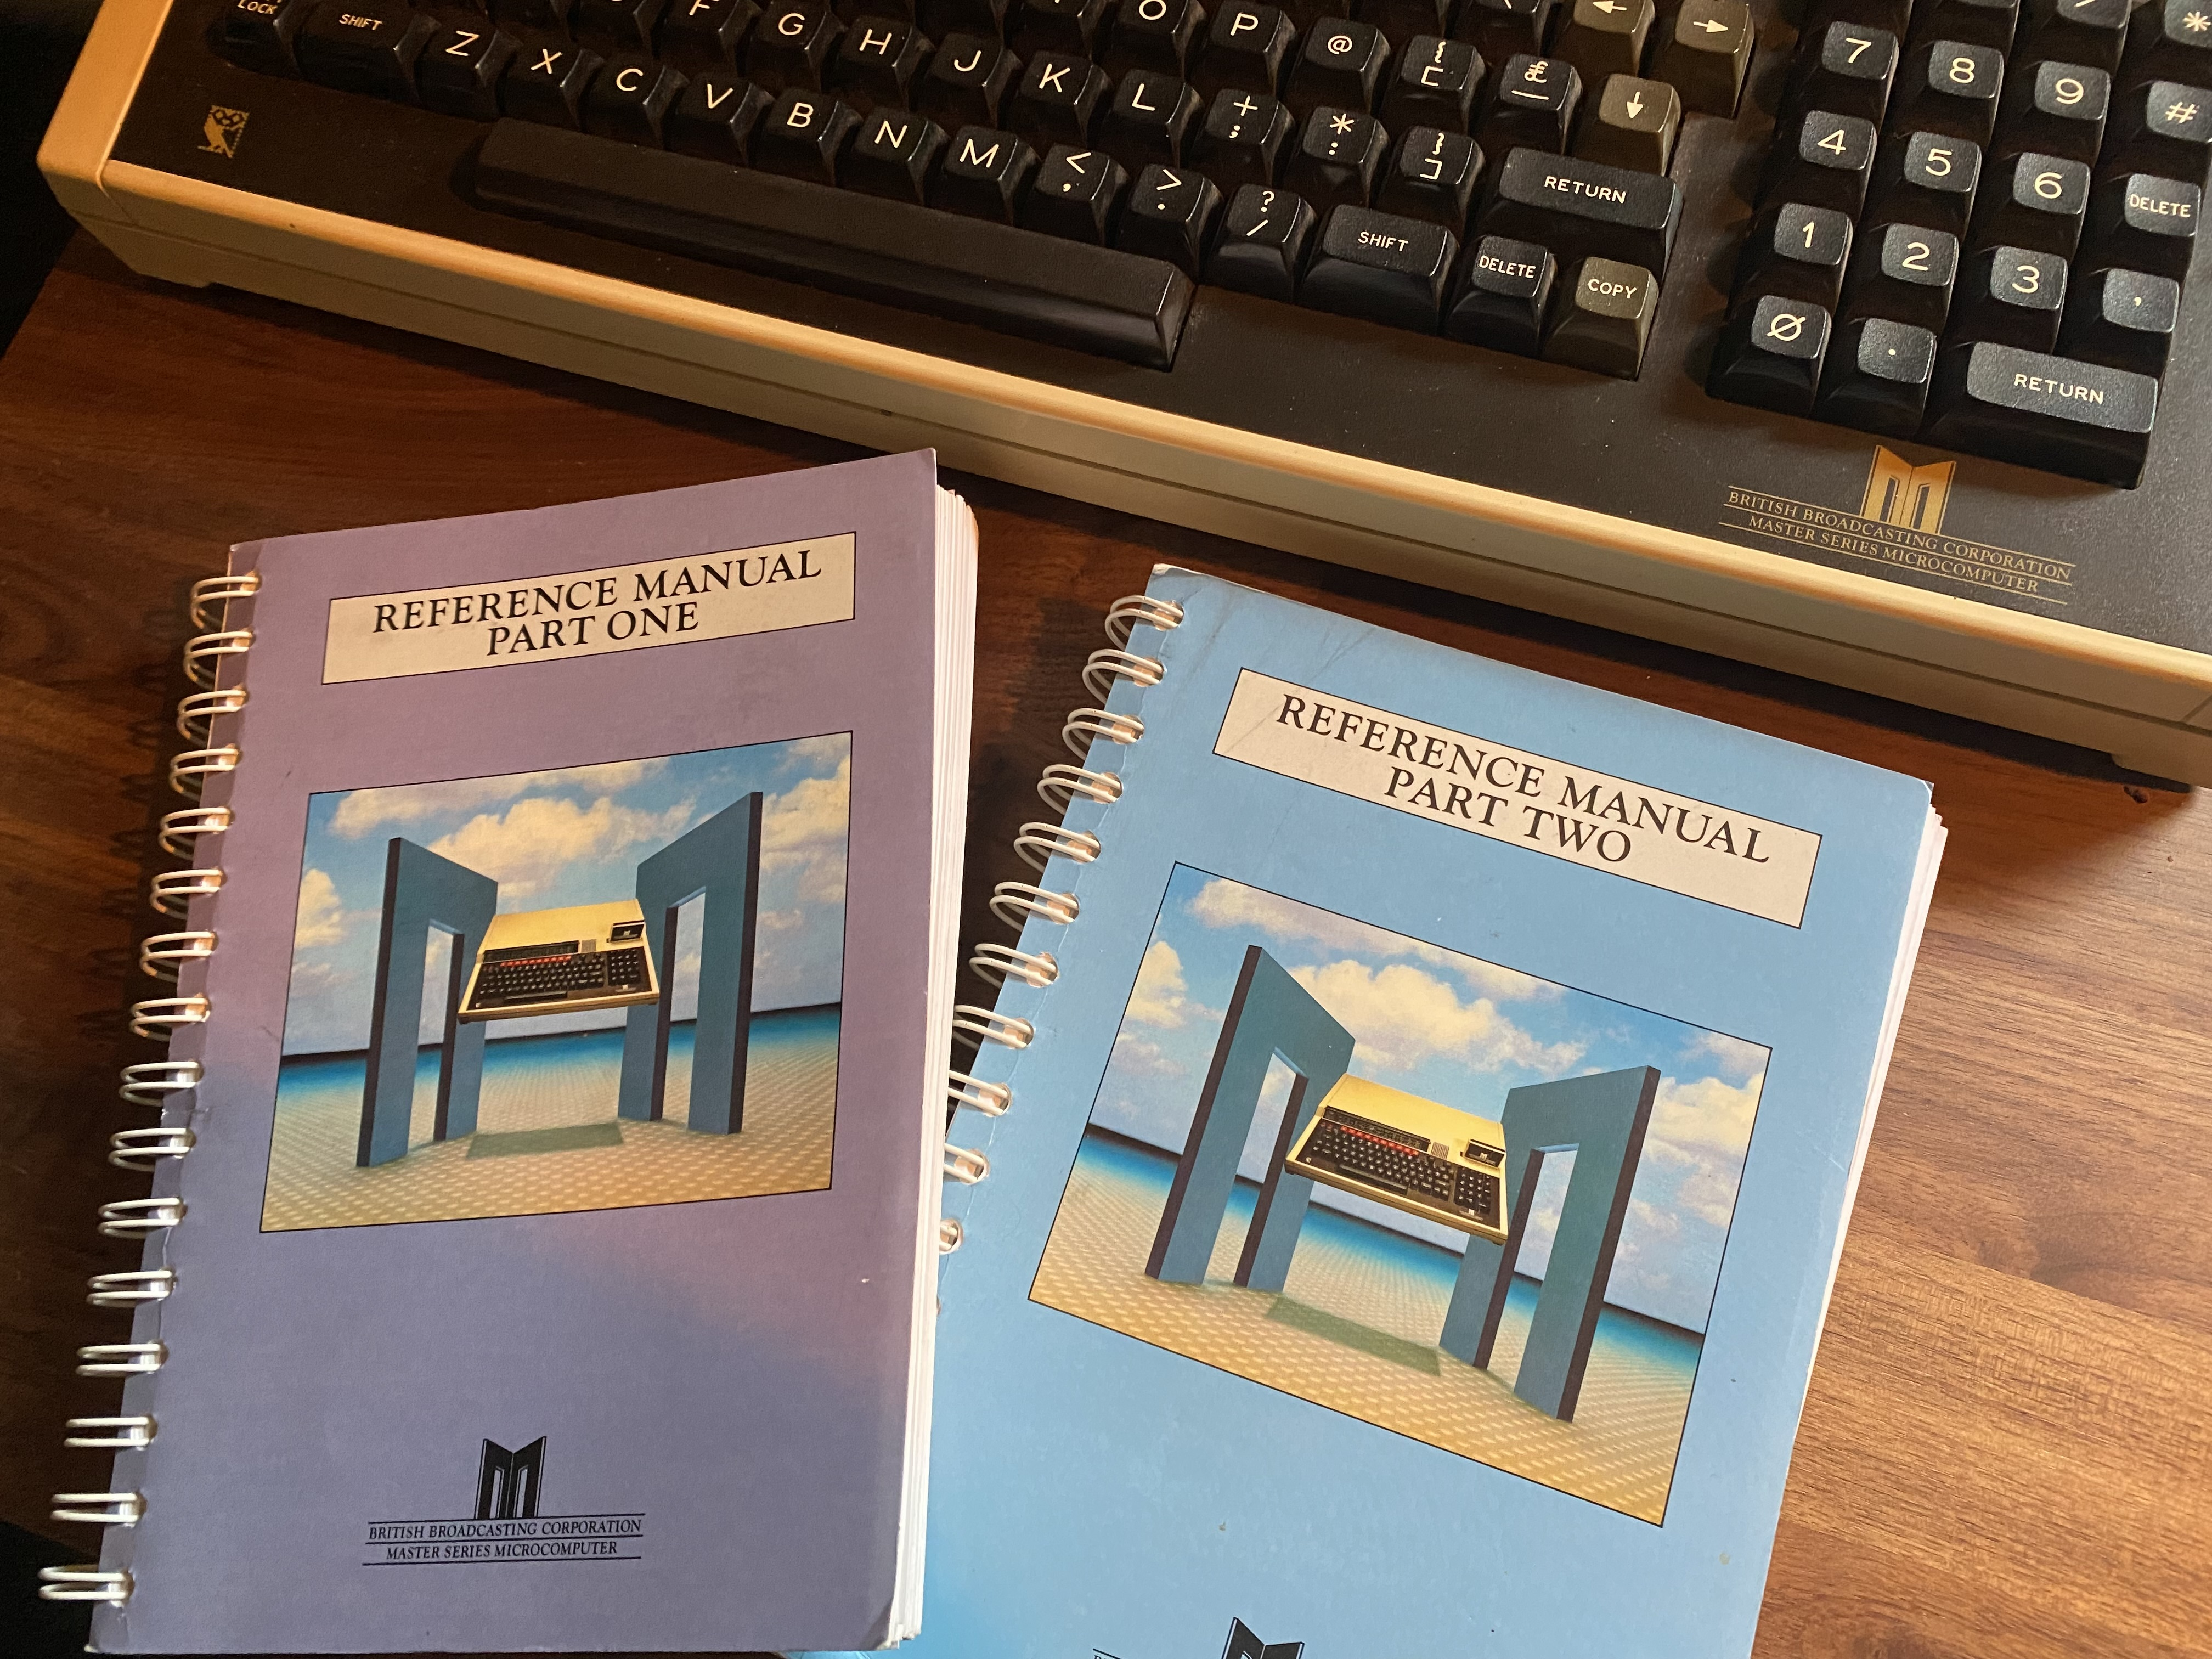
\includegraphics[height=3cm]{Photo 08-02-2022, 11 46 37.jpg}\\
\scriptsize{\emph{A photo of my own reference manuals.}}
\end{center}
\par{This is where the \DARIC{} story really begins. The \emph{Beeb} as it's affectionally known, is a very capable machine for programming. The BASIC supported structured programming, with procedures, local variables and inline macro assembler. It supported plugin ROMs, similar to cartridges. These ROMs enabled additional applications and programming languages to be available immediately from power-on, such as LISP, FORTH etc.}
\par{Inspired by these languages and INPUT magazine (of which I owned every issue), I started to write my own programming language. I named it ASPL - Advanced Structured Programming Language. Arguably the first two words were not appropriate, but I had visions of grandeur.}

\subsection{Compilation, interpreting and machine code}
\par{This is probably a good time to talk about machine code, and why effort was put in to learn it.}
\par{Machine code is the language of the computer itself. By talking this language, it's possible to eek out the maximum possible performance. But this comes at a cost, it's difficult to learn and even more difficult to successfully use. There are no \emph{real} numbers (i.e. numbers with decimal places), there are no strings, there is no multiply or divide, everything has to be coded in terms of simple opcodes. Some master this, but even for them it's still slower than using a higher level language like BASIC.}
\par{Languages such as BASIC were typically \emph{interpreted}, a special program called an interpreter would execute the program. This was much slower than machine code, but had distinct interactive advantages, such as iterative development - building a program up piece by piece.}
\par{What I wanted was ASPL to have the advantages of a high level language, but compiled to machine code. A \emph{compiler}. I mostly achieved this goal, but the generated code was far from optimal. I understand the concepts of optimisation, but had no practical experience. This was pre-internet, it wasn't easy to learn except through books.}
\par{That is where the ASPL story ended. For around 30 years, and then I was re-inspired to revisit it. This time it had a different name, PiBASIC.}

\section{PiBASIC and the PiTubeDirect}
\par{There is a wonderful piece of hardware called the Tube on a BBC Micro. It allows co-processors to be used, as parasite with the Beeb as a host, using its I/O. When the machine was at its zenith, there were a variety of external co-processors available, such as a 32016, Z80, or an additional 6502 processor.}
\par{The very first ARM chip was also created as a co-processor for the BBC Micro.}
\par{The PiTubeDirect uses a Raspberry Pi to emulate all of these co-processors, enabling the humble Beeb to run at huge speed due to the modern ARM chip. It's sort of fitting really. What interested me is the \emph{Native} ARM mode - the ability to run ARM code at a 1000MHz inside a Beeb.}
\par{I started work on PiBASIC, a BBC BASIC compatible interpreter, but which supported VFP instructions for hardware floating point maths. I wanted to recreate Zarch on the BBC Micro. A project that is still on the back burner today!}
\par{The original version was written in C, using the open-source Flex \& Bison for parsing source. By the third major rewrite it was running on my Linux machine for faster development, by the 5th iteration it was using Antlr for source parsing, and it was written in C++.}
\par{Around this time the name change occurred, and I started to use LLVM - a compiler library for outputting native machine code. There were a few iterations before settling on V14, the version it is now. A command line compiler that outputs an executable file.}

\section{\DARIC}
\par{\DARIC{} is cross-platform, runs on Windows, macOS and Linux.}
\par{\DARIC{} is built on the following technology:}
\begin{itemize}
\item Written in modern \CC - safe, performant and cross-platform.
\item LLVM - outputs X64 or ARM64 machine code. 
\item Antlr4 - powerful and modern parser, allows quick syntax changes. 
\item SDL2 - cross-platform window management and 2D. 
\item OpenGL3 - hardware accelerated 3D.
\item Dear ImGui - UI library.
\item Assimp - 3D asset loading.
\end{itemize}
\par{All of this technology is hidden behind a simple BASIC syntax, the \DARIC{} compiler does all the hard work making it all happen.}

\section{Who is the sloth?}
A very capable designer friend of mine created the logo, the sloth is chilled, happy and in no rush.
\begin{center}

\includegraphics[height=3cm]{2021-DARIC-SECONDARYLOGO-CIRCULARICON-BLACK.png}\\
\scriptsize{\emph{The \DARIC{} mascot!}}
\end{center}
\chapter{Getting and running \DARIC}

\section{Downloading \DARIC}

\section{The \emph{Welcome Tape}}

\chapter{Learning \DARIC}

\section{Conventions}
\par{There are a some conventions from here on. A block of \DARIC{} code looks like this:}
\example{
	PRINT 1543.45+SQR(4.6)-12.42
}
{The output displayed on screen looks like this:}
\out{
	1533.17476106
}

\section{The PRINT statement}
\par{Let's learn some \DARIC{}! There is something called 'Hello, World!' which is a simple program to introduce a programming language. Type the following into a text file using an editor of your choice:}
\example{
	PRINT "Hello, world!"
}
\par{Compile and run the resulting executable - your first program!}
\out{
	Hello, world!
}
\par{If you've programmed before you probably aren't too impressed, but it still means everything is working as it's supposed to.}
\par{What is important here, is that your program is creating a window, starting up OpenGL graphics and then rendering the text to a \emph{console}, all automatically. If you repeat the \emph{PRINT} statement enough times it will scroll the screen. You'll see later that this \emph{console} sits on top of other graphics you draw.}
\par{Let's display some numbers as well as text.}
\example{
	PRINT "Hello, world!"\\
	PRINT 123.45\\
	PRINT 100,100;100
}
\par{What does that give us? Run it and see.}
\out{
	Hello, world!\\
	123.45\\
	100     100100
}
\par{What is happening here? The first is the use of a comma and semicolon in the \emph{PRINT} statement, this is output formatting and covered in \autoref{sec:PRINT} on page \pageref{sec:PRINT}.}
\par{Secondly, we are printing three different literal values. This is covered in the next section.}

\section{Integers, floats and strings}
\par{A literal is a constant, exact value, like the number 100 or the text "string". \DARIC{} supports three different types:}
\begin{itemize}
\item Integers - these are whole numbers, no decimal/fractional part. In \DARIC{}, they are represented by 64bit integers.
\item Floats - these are real numbers, and can represent numbers with a decimal part. in \DARIC{}, these are represented by double precision 64bit floats. 
\item Strings - defined as a \emph{string} of zero or more ASCII characters.
\end{itemize}
\par{Some programming languages support many more, but \DARIC{} keeps it simple.}
\par{It's possible to do lots of things with literals without ever storing the result, such as calculations:}
\example{
	PRINT 1543.45+SQR(4.6)-12.42
}
\out{
	1533.17476106
}
\par{But let's be honest, this isn't particularly useful. Unless of course we want to just pretend it's a fancy calculator.}
\par{To do something useful, we need to \emph{store} these values somewhere.}

\section{Variables}
\section{Loops}
\section{Control statements}
\section{Procedures}
\section{Arrays}
\section{DATA and READ}
\section{Structured types}
\section{Object-oriented programming (OOP)}
\chapter{2D Graphics}
\section{Drawing primitives}
\section{Colour, foreground and background}
\section{Sprites}
\chapter{3D Graphics}
\section{Creating a 3D model}
\section{Moving, rotating and scaling 3D models}
\section{What is the camera?}
\label{sec:Camera}
This is some text.
\section{Loading meshes}
\chapter{Sound}
\chapter{Keyword Reference}
\chapter{API Reference}

\section{2D Graphics}

\label{sec:PRINT}

\lrefi
{CIRCLE}{Circle}{circle}
{Statement drawing an outlined circle of the specified radius at the specific point on screen.}
{\opo{}x\tr,y\tr,r\tr\otr{w}\opc{}}
{The parameters specify the screen co-ordinate and the radius (in pixels).
\begin{itemize}
\item If the 5th optional parameter isn't specified, it's a 1px wide outlined circle - but scaled depending on whether a \emph{logical} resolution is set.
\item If the 5th optional parameter \emph{is} specified, it specifies the outline width but scaled as above. 
\end{itemize}}
{CIRCLE 350,150,50,2.5}
{}

\lref
{CIRCLEFILL}{CircleFill}{circlefill}
{Statement drawing a filled circle of the specified radius at the specific point on screen. The current foreground colour is the fill colour.}
{\opo{}x\tr,y\tr,r\tr\opc{}}
{The parameters specify the screen co-ordinate and the radius (in pixels).}
{CIRCLEFILL 640,240,80}
{}

\lref
{CLIPON}{ClipOn}{clipon}
{Statement enabling clipping of graphics drawing. All 2D drawing operations will clip to this bounding box. Multiple calls are not recommended and a \emph{CLIPOFF} is needed to restore normal operation.}
{\opo{}x1\tr,y1\tr,x2\tr,y2\tr\opc{}}
{The first two parameters specify the upper-left corner, the last two the lower-right corner.}
{CLIPON 100,200,500,500}
{}

\lref
{CLIPOFF}{ClipOff}{clipoff}
{Statement cancelling the current clipping operation. All 2D drawing operations will return to normal after this statement.}
{\opo{}\opc{}}
{}
{CLIPOFF 100,200,500,500}
{}

\lref
{CLS}{Cls}{cls}
{Statement clearing the screen: text and graphics, and resets the cursor position.}
{\opo{}\opc{}}
{}
{CLS}
{}

\lref
{CURSORON}{CursorOn}{cursoron}
{Statement showing the flashing text cursor. If already flashing, does nothing.}
{\opo{}\opc{}}
{}
{CURSORON}
{}

\lref
{CURSOROFF}{CursorOff}{cursoroff}
{Statement hiding the flashing text cursor. If already hidden, does nothing.}
{\opo{}\opc{}}
{}
{CURSOROFF}
{}

\lref
{FLIP}{Flip}{flip}
{When in \emph{BANKED} mode, this statement will flip the backbuffer to screen. In \emph{CLASSIC} mode, it does nothing. This allows lots of graphical changes to be made and only shown when ready. The user won't see the screen being drawn in parts.}
{\opo{}\opc{}}
{}
{FLIP}
{}

\lrefi
{LINE}{Line}{line}
{Statement drawing a line between two points on screen.}
{\opo{}x1\tr,y1\tr,x2\tr,y2\tr\otr{w}\opc{}}
{These parameters specify the start and end screen co-ordinates.
\begin{itemize}
\item If the 5th optional parameter isn't specified, it's a 1px wide line - but scaled depending on whether a \emph{logical} resolution is set.
\item If the 5th optional parameter \emph{is} specified, it specifies the line width but scaled as above. 
\end{itemize}}
{LINE 100,150,300,250}
{}

\lref
{MODE}{Mode}{mode}
{Statement changing the current graphics mode as specified and clears screen. This also affects text drawing. This switches drawing into \emph{CLASSIC} mode, i.e. all graphics and text operations appear immediately.}
{\opo{}w\ti,h\ti,lw\ti,lh\ti\opc{}}
{\par{The first two parameters specify the desired width and height, the last two parameters specify the logical width and height. Typically these are the same values to give a direct mapping of screen co-ordinates.}
\par{This can be used for instance to emulate the logical screen resolution of the BBC Micro, the following will give a MODE 0 equivalent resolution:}
\par{\codec{MODE 640,256,1280,1024}}
\par{Or it could be used to allow drawing to a fixed resolution, but which scales to the physical screen resolution:}
\par{It's also possible to use -1 as a parameter, this will default to the current desktop resolution in that parameter position.}}
{MODE SCREENWIDTH(),SCREENHEIGHT(),1280,720}
{}

\lref
{MODEB}{ModeB}{modeb}
{Statement changing the current graphics mode as specified and clears screen. This also affects text drawing. This switches drawing into \emph{BANKED} mode, i.e. double buffered.}
{\opo{}w\ti,h\ti,lw\ti,lh\ti\opc{}}
{These parameters are the same as for the \emph{MODE} statement.}
{MODEB -1,-1,-1,-1}
{}

\lref
{PLOT}{Plot}{plot}
{Statement plotting a pixel in the current foreground colour.}
{\opo{}x\tr,y\tr\opc{}}
{The two parameters specify the co-ordinate of the pixel to plot.}
{PLOT 120,450}
{}

\lref
{RECTANGLE}{Rectangle}{rectangle}
{Statement drawing a rectangle between two points on screen. The current foreground colour is used.}
{\opo{}x1\tr,y1\tr,x2\tr,y2\tr\opc{}}
{These parameters specify the start and end screen x \& y co-ordinates.}
{RECTANGLE 200,200,300,450}
{}

\lref
{FILLEDRECTANGLE}{FilledRectangle}{filledrectangle}
{Statement drawing a filled rectangle between two points on screen. The current foreground colour is used for the fill.}
{\opo{}x1\tr,y1\tr,x2\tr,y2\tr\opc{}}
{\par{These parameters specify the start and end screen x \& y co-ordinates.}}
{FILLEDRECTANGLE 200,200,300,450}
{}

\lref
{SCREENWIDTH}{ScreenWidth}{screenwidth}
{Function returning the current desktop screen width. Commonly used as part of a \emph{MODE} or \emph{MODEB} statement.}
{\opo{}\opc{}}
{}
{w\%=SCREENWIDTH()}
{\tri{}}

\lref
{SCREENHEIGHT}{ScreenHeight}{screenheight}
{Function returning the current desktop screen height. Commonly used as part of a \emph{MODE} or \emph{MODEB} statement.}
{\opo{}\opc{}}
{}
{h\%=SCREENHEIGHT()}
{\tri{}}

\lref
{TRIANGLE}{Triangle}{triangle}
{Statement drawing an outlined triangle between three points on screen. The current foreground colour is used.}
{\opo{}x1\tr,y1\tr,x2\tr,y2\tr\,x3\tr,y3\tr\opc{}}
{These parameters specify the start and end screen x \& y co-ordinates for all three points.}
{TRIANGLE 50,50,150,100,75,200}
{}

\lref
{TRIANGLEFILL}{TriangleFill}{trianglefill}
{Statement drawing a filled triangle between three points on screen. The current foreground colour is used for the fill.}
{\opo{}x1\tr,y1\tr,x2\tr,y2\tr\,x3\tr,y3\tr\opc{}}
{These parameters specify the start and end screen x \& y co-ordinates for all three points.}
{TRIANGLEFILL 50,50,150,100,75,200}
{}

\lref
{TRIANGLESHADED}{TriangleShaded}{triangleshaded}
{Statement drawing a shaded triangle between three points on screen. 
Each vertex (corner) can be a different colour and the fill pixel colours are blended from these.}
{\opo{}x1\tr,y1\tr,x2\tr,y2\tr\,x3\tr,y3\tr\opc{}}
{These parameters specify the start and end screen x \& y co-ordinates and the vertex colour (as an RGB integer) for all three points.}
{TRIANGLESHADED 50,50,\&0000FF,150,100,\&00FF00,75,200,\&FF0000}
{}

\section{3D Graphics}

\lref
{CAMERA}{Camera}{camera}
{Statement setting the position of the 3D camera.}
{\opo{}x\tr,y\tr,z\tr,rx\tr,ry\tr,rz\tr,lx\tr,ly\tr,lz\tr\opc{}}
{This statement sets the 3D camera, both the position, the rotation (think twisting the camera), and the position being looked at. This is all explained in \autoref{sec:Camera}{\emph{ (What is the camera?)}} on page \pageref{sec:Camera}.}
{CAMERA 0,4,-10,0,0,0,0,0,0}
{}

\lref
{DELETEOBJECT}{DeleteObject}{deleteobject}
{Statement deleting an object.}
{\opo{}id\opc{}}
{The parameter specified a handle previously returned from a \emph{OBJECT} function call. The object will be removed from the 3D scene on the next \emph{RENDER}.}
{DELETEOBJECT \%spaceship}
{}

\lref
{DELETESHAPE}{DeleteShape}{deleteshape}
{Statement deleting a shape.}
{\opo{}id\opc{}}
{The parameter specified a handle previously returned from a \emph{SHAPE} function call. This call needs to be used with caution, deleting a shape that is used by \emph{OBJECT}s will cause undefined behaviour.}
{DELETESHAPE \%shape1}
{}

\lref
{FACE}{Face}{face}
{Statement creating a triangle face.}
{\opo{}vertex1\ti,vertex2\ti,vertex3\ti\oti{colour}\opc{}}
{This statement creates a 3D face and adds to the list of faces to create a shape with. The first three parameters \emph{vertex1,vertex2,vertex3} specify each index of the three vertices (corners) - remember that in \DARIC, indices always start from 1 and not 0. The optional \emph{colour} parameter gives the face an RGB colour typically created with the \emph{COL} function. If no colour is assigned, then a gouraud shaded face will be created, i.e. a face which is smooth shaded between the colours at the three vertices.}
{FACE 4, 2, 1}
{}

\lref
{LOADMESH}{LoadMesh}{loadmesh}
{Statement creating a vertex (corner of a shape).}
{\opo{}filename\ts\opc{}}
{This function loads a 3D mesh from a file and returns the handle of a shape. It uses the \emph{assimp} library to load supported file types. Common formats such as Blender, and 3D Studio are supported. See \url{https://github.com/assimp/assimp/blob/master/doc/Fileformats.md} for a complete list.}
{tree\%=LOADMESH("tree.obj")}
{\tri{}}

\lref
{OBJECT}{Object}{object}
{Function creating a 3D object.}
{(id\ti,x\tr,y\tr,z\tr,rx\tr,ry\tr,rz\tr,\allowbreak{}scale\tr,\allowbreak{}type\ti)}
{\par{The first three parameters \emph{x,y,z} specify the location of the object in 3D space. The next 3 \emph{rx,ry,yz} specify the rotation of the object. The \emph{scale} parameter specifies how large the object is compared to the base 3D shape, 1.0 would render at the same size as the shape.}
\par{The \emph{type} specifies the type of the object:}
\par{0 - Solid, this is a fully shaded object.}
\par{1 - Wireframe, i.e. the outline of an object is drawn. Hidden lines are removed.}
\par{2 - Filled Wireframe, the outline of an object is drawn in the current foreground colour, but the polygons are also filled with colour.}}
{obj\%=OBJECT(spaceship\%,10.5,12.2,130.9,30,120,60,1.0,0)}
{\tri{}}

\lref
{RENDER}{Render}{render}
{This statement renders the current 3D scene.}
{\opo{}\opc{}}
{}
{RENDER}
{}

\lref
{ROTATE}{Rotate}{rotate}
{Statement that causes a 3D object to be rotated.}
{\opo{}id\ti,x\tr,y\tr,z\tr\opc{}}
{This statement rotates an existing 3D object. The first parameter \emph{id} is the shape handle returned from \emph{SHAPE}. The next three parameters \emph{x,y,z} specify the new rotation in degrees for each axis.}
{ROTATE bullet\%,30,90,45}
{}

\lref
{SCALE}{Scake}{scale}
{Statement that causes a 3D object to be scaled (resized).}
{\opo{}id\ti,scale\tr\opc{}}
{This statement scales an existing 3D object. The first parameter \emph{id} is the shape handle returned from \emph{SHAPE}. The next parameter \emph{scale} specifies the new scale of the 3D object.}
{SCALE ship\%,2}
{}

\lref
{SHAPE}{Shape}{shape}
{Statement creating a shape.}
{()}
{This function uses a list of vertices and faces that have been added with the \emph{VERTEX} and \emph{FACE} statements. It creates a new shape, returns the handle and clear the vertices and face list.}
{
REM ** Build vertices **\\
VERTEX -0.5,  0.5,  0.5, 0\\
VERTEX  0.5,  0.5,  0.5, 0\\
VERTEX  0.5, -0.5,  0.5, 0\\
VERTEX -0.5, -0.5,  0.5, 0\\
VERTEX -0.5,  0.5, -0.5, 0\\
VERTEX  0.5,  0.5, -0.5, 0\\
VERTEX  0.5, -0.5, -0.5, 0\\
VERTEX -0.5, -0.5, -0.5, 0\\
\\
REM ** Build triangle faces **\\
col\%=\&FF0000\\
FACE 4, 2, 1, col\%:FACE 4, 3, 2, col\%:REM Front\\
FACE 6, 7, 8, col\%:FACE 6, 8, 5, col\%:REM Back\\
FACE 4, 8, 7, col\%:FACE 4, 7, 3, col\%:REM Top\\
FACE 5, 1, 2, col\%:FACE 6, 2, 5, col\%:REM Bottom\\
FACE 5, 8, 4, col\%:FACE 5, 4, 1, col\%:REM Left\\
FACE 2, 3, 7, col\%:FACE 2, 7, 6, col\%:REM Right\\
cube\%=SHAPE()
}
{\tri{}}

\lref
{TRANSLATE}{Translate}{translate}
{Statement that causes a 3D object to be translated (moved).}
{\opo{}id\ti,x\tr,y\tr,z\tr\opc{}}
{This statement translates an existing 3D object. The first parameter \emph{id} is the shape handle returned from \emph{SHAPE}. The next three parameters \emph{x,y,z} specify the new position in 3D space.}
{TRANSLATE ship\%,5,0,10}
{}

\lref
{VERTEX}{Vertex}{vertex}
{Statement creating a vertex (corner of a shape).}
{\opo{}x\tr,y\tr,z\tr,colour\ti\opc{}}
{This statement creates a 3D vertex and adds to the list of vertices to create a shape with. The first three parameters \emph{x,y,z} specify the local co-ordinate of the vertex. The centre of the shape is 0,0,0. The \emph{colour} parameter gives the vertex an RGB colour typically created with the \emph{COL} function. }
{VERTEX -0.5,  0.5,  0.5, \&FF00FF}
{}

\section{Chrono}

\lref
{TIME}{Time}{time}
{Function that returns the number of centiseconds since the program started running.}
{()}
{}
{t=TIME()}
{\tri}

\lref
{TIME\$}{Time\$}{time\$}
{Function returning the current time in a format like: Sun,02 Feb 2003.18:33:30.}
{()}
{}
{PRINT TIME\$()}
{\tri}

\section{Colour}

\lref
{BG}{Bg}{bg}
{This statement sets the current background drawing colour.}
{\opo{}r\ti,g\ti,b\ti\opc{}}
{The three parameters \emph{r,g,b} specify the red, green and blue components in the range 0-255.}
{BG(\&10,\&10,\&10)}
{}

\lref
{COL}{Col}{col}
{This function returns the RGB value, including alpha channel.}
{\opo{}r\ti,g\ti,b\ti,\oti{a}\opc{}}
{The three parameters \emph{r,g,b} specify the red, green and blue components in the range 0-255. The optional \emph{a} specified the alpha channel component, if not specified then 255 is assumed.}
{col\%=COL(\&FF,\&0,\&FF)}
{}

\lreftwo
{FG}{Fg}{fg}
{This statement sets the current foreground drawing colour.}
{\opo{}r\ti,g\ti,b\ti,\oti{a}\opc{}}
{\opo{}rgb\ti\opc{}}
{
\par{There are two versions of this function, one taking separate RGB[a] values, and the other taking a single RGB value.}
\par{For the first version there are three parameters \emph{r,g,b} specify the red, green and blue components in the range 0-255. The optional \emph{a} specifies the alpha channel component, if not specified then 255 is assumed.}
}
{FG \&FF,\&FF,\&FF\\FG \&FF0000}
{}

\section{File I/O}

\lref
{BGET\#}{BGet\#}{bget\#}
{Function that reads a single byte from a file.}
{(channel\ti)}
{The \emph{channel} handle is a file previously opened with \emph{OPENIN}.}
{B\%=BGET\#(channel\%)}
{\tri}

\lref
{BPUT\#}{BPut\#}{bput\#}
{Statement that write a single byte to a file.}
{(channel\ti,byte\ti)}
{The \emph{channel} handle is a file previously opened with \emph{OPENIN}.}
{BPUT\#(channel\%,ASC("A"))}
{}

\lref
{CLOSE\#}{Close\#}{close\#}
{Statement that closes a file channel.}
{(channel\ti)}
{The \emph{channel} handle is a file previously opened with \emph{OPENIN},\emph{OPENOUT} or \emph{OPENUP}.}
{CLOSE\#(channel\%)}
{}

\lref
{EOF\#}{Eof\#}{eof\#}
{A function to test for end of file (EOF).}
{(channel\ti)}
{The \emph{channel} handle is a file previously opened with \emph{OPENIN}. This function returns a 0 or 1 depending on whether end-of-file has been reached or not.}
{REPEAT UNTIL EOF\#(channel)}
{\tri}

\lref
{GET\$\#}{Get\$\#}{get\$\#}
{A function to read an entire line from a file.}
{(channel\ti)}
{The \emph{channel} handle is a file previously opened with \emph{OPENIN}. The function returns a string. It's best to check for end-of-file first.}
{l\$=GET\$\#(channel\%)}
{\trs}

\lref
{OPENIN}{OpenIn}{openin\#}
{Function that opens a file for reading.}
{(filename\ts)}
{The filename should exist before calling the function, otherwise the program will end with an error. It returns a file handle.}
{channel\%=OPENIN("Filename.txt")}
{\tri}

\lref
{OPENUP}{OpenUp}{openup\#}
{Function that opens a file for appending (i.e. adding to the end of the file).}
{(filename\ts)}
{The filename should exist before calling the function, otherwise the program will end with an error. It returns a file handle.}
{channel\%=OPENUP("Filename.txt")}
{\tri}

\lref
{OPENOUT}{OpenOut}{openout\#}
{Function that opens a file for writing.}
{(filename\ts)}
{The file is opened for writing. If it already exists, then the contents will be truncated. It returns a file handle.}
{channel\%=OPENOUT("Filename.txt")}
{\tri}

\lref
{PTR\#}{Ptr\#}{ptr\#}
{Function that retrieves the current read\&write position in the file.}
{(channel\ti)}
{The \emph{channel} handle is a file previously opened with \emph{OPENIN},\emph{OPENOUT} or \emph{OPENUP}. It returns the current read\&write pointer, with 0 being start of file.}
{p\%=PTR\#(channel\%)}
{\tri}

\lref
{SPTR\#}{SPtr\#}{sptr\#}
{Statement that moves the read\&write position in the file.}
{(channel\ti,position\ti)}
{The \emph{channel} handle is a file previously opened with \emph{OPENIN},\emph{OPENOUT} or \emph{OPENUP}. The \emph{position} should be valid, otherwise the program will end with an error.}
{SPTR\#(channel\%,1000)}
{}

\section{Mouse \& Keyboard}

\lref
{INKEY}{Inkey}{inkey}
{Function returning a keycode, or checking a specific key is pressed.}
{(value\ti)}
{This function works in two modes, depending on what is passed as parameter \emph{value}.
\begin{itemize}
\item If the parameter is -1 or less, then INKEY checks for a specific key being pressed. Take the key code, add 1 and make the number negative (so the Space Bar, code 98, becomes -99). Returns 1 if the key is currently being pressed, 0 otherwise.
\item If the parameter is 0 or more then INKEY waits the specified centiseconds for a keypress. Returns the ASCII code if the key is pressed before the end of the timeout, otherwise returns -1.
\end{itemize}

The key codes are covered in \autoref{sec:INKEY}{\emph{ (INKEY Key Codes)}} on page \pageref{sec:INKEY}.}
{\parbox{\textwidth}{
IF INKEY(-99) PRINT "Space pressed"\\
IF INKEY(100)=-1 PRINT "Timeout"}}
{\tri}

\lref
{INKEY\$}{Inkey\$}{inkey\$}
{Function returning a string of the key pressed.}
{(timeout\ti)}
{The parameter \emph{timeout} is 0 or more and specifies the wait in centiseconds, similar to INKEY. It returns a string of length 1 with the key pressed, such as "A" if a key is pressed before the timeout, otherwise returns an empty string.}
{IF INKEY\$(100)="A" PRINT "A Pressed"}
{\trs}

\lref
{GET}{Get}{get}
{Function waiting for a key press and returning the keycode.}
{()}
{It returns the ASCII code of the next key pressed (or already pressed and in the buffer). It will wait for a key to be pressed.}
{IF GET()=32 PRINT "Space pressed"}
{\tri}

\lref
{GET\$}{Get\$}{get\$}
{Function waiting for a key press and returning the character.}
{()}
{It returns the next key pressed (or already in the buffer) as a 1 character string. It will wait for a key to be pressed.}
{IF GET\$="Z" PRINT "Yes!"}
{\trs}

\lref
{MOUSEX}{MouseX}{mousex}
{Function returning the current X position of the mouse pointer.}
{()}
{}
{x\%=MOUSEX()}
{\tri}

\lref
{MOUSEY}{MouseY}{mousey}
{Function returning the current Y position of the mouse pointer.}
{()}
{}
{y\%=MOUSEY()}
{\tri}

\lref
{MOUSESTATE}{MouseState}{mousestate}
{Function returning the current state of the mouse buttons.}
{()}
{
\par{This returns an integer value representing all 3 mouse buttons - each button being a single bit combined to show the state of all 3 buttons.}
\par{Button 1 (left) is value 4, button 2 (middle) is value 2 and button 3 (right) is value 1.\\\\By using the logical AND operator it's possible to get the state of each.}
}
{buttons\%=MOUSESTATE():IF buttons\% AND 4 PRINT "Left pressed"}
{\tri}

\section{Maths Functions}

\lref
{ACS}{Acs}{acs}
{Function returning the arc-cosine.}
{(expr\tr)}
{The parameter \emph{expr} is a real number between -1 and 1 inclusive. It returns a real in the range 0 to PI radians.}
{ang\#=ACS(0.5)}
{\trr}

\lref
{ASN}{Asn}{asn}
{Function returning the arc-sine.}
{(expr\tr)}
{The parameter \emph{expr} is a real number between -1 and 1 inclusive. It returns a real in the range -PI/2 to PI/2 radians.}
{ang\#=ASN(0.5)}
{\trr}

\lref
{ATN}{Atn}{atn}
{Function returning the arc-tangent.}
{(expr\tr)}
{The parameter \emph{expr} is a real number between -1 and 1 inclusive. It returns a real in the range -PI/2 to PI/2 radians.}
{PRINT ATN(opp/adj)}
{\trr}

\lref
{COS}{Cos}{cos}
{Function returning the cosine.}
{(expr\tr)}
{The parameter \emph{expr} is an angle in radians between -PI/2 and PI/2, numbers outside this range are scaled down to the range. It returns a real in the range -1 to 1 radians.}
{PRINT COS(RAD(30))}
{\trr}

\lref
{DEG}{Deg}{deg}
{Function converting from radians to degrees.}
{(expr\tr)}
{The parameter \emph{expr} is an angle in radians between -PI/2 and PI/2, numbers outside this range MAY work. It returns the number of degrees, calculated with 180*\emph{expr}/PI.}
{PRINT DEG(PI()/2)}
{\trr}

\lref
{EXP}{Exp}{exp}
{Function returning the exponent.}
{(expr\tr)}
{This function returns the exponent of the parameter \emph{expr}. This is e raised to the power of \emph{expr}.}
{a\#=EXP(3.2)}
{\trr}

\lref
{LN}{Ln}{ln}
{Function returning the natural logarithm.}
{(expr\tr)}
{This function returns the natural logarithm of the parameter \emph{expr}.}
{PRINT LN(10)}
{\trr}

\lref
{LOG}{Log}{log}
{Function returning the logarithm to base 10 of its numeric argument.}
{(expr\tr)}
{This function returns the natural logarithm to base 10 of the parameter \emph{expr}. This will not return 0.}
{a\#=LOG(2.476)}
{\trr}

\lref
{PI}{Pi}{pi}
{Function returning the value of PI.}
{()}
{This function returns a real representing PI to the accuracy offered by a double precision floating point number.}
{a\#=SIN(RAD(135))*PI()}
{\trr}

\lref
{RAD}{Rad}{rad}
{Function returning the value of the argument (specified in degrees) in radians.}
{(expr\tr)}
{Returns a real giving the angle in radians, for the angle in degrees parameter \emph{expr}.}
{r\#=RAD(270)}
{\trr}

\lref
{SGN}{Sgn}{sgn}
{Function giving the sign of its numeric argument.}
{(expr\tr)}
{Returns -1 if \emph{expr} is negative, 0 if \emph{expr} is zero or 1 otherwise.}
{IF SGN(A)=1 THEN PROCPos()}
{\tri}

\lref
{SIN}{Sin}{sin}
{Function returning the sine.}
{(expr\tr)}
{The parameter \emph{expr} is an angle in radians between -PI and PI, numbers outside this range are scaled down to the range. It returns a real in the range -1 to 1 radians.}
{PRINT SIN(RAD(135))}
{\trr}

\lref
{SQR}{Sqr}{sqr}
{Function returning the square root of the numeric argument.}
{(expr\tr)}
{Returns a real giving the square root of \emph{expr}.}
{a\#=b\# + SQR(h\# * l\#)}
{\trr}

\lref
{TAN}{Tan}{tan}
{Function returning the tangent.}
{(expr\tr)}
{The parameter \emph{expr} is an angle in radians between -PI/2 and PI/2, numbers outside this range are scaled down to the range. It returns a real.}
{PRINT TAN(RAD(theta\#))}
{\trr}

\section{Random Numbers}

\lref
{RND}{Rnd}{rnd}
{Function returning an integer random number.}
{(expr\ti)}
{This function returns an integer random number in the range 0 to parameter \emph{expr} inclusive.}
{t\%=RND(100)}
{\trr}

\lref
{RNDF}{RndF}{rndf}
{Function returning a real random number.}
{(expr\tr)}
{This function returns a reak random number in the range 0 to parameter \emph{expr} inclusive.}
{t\#=RND(6.5)}
{\trr}

\section{Sprites}

\lref
{CREATESPRITE}{CreateSprite}{createsprite}
{Function creating a sprite by grabbing a portion of the screen.}
{(x\ti,y\ti,w\ti,h\ti)}
{The first parameters \emph{x,y} specifies the position onscreen to grab, the \emph{w,h} parameters specify the size of the area to grab and the size of the resulting sprite. If running in \emph{BANKED} mode, then a \emph{FLIP} may be required first. It returns a sprite handle.}
{drone\%=CREATESPRITE(100,100,50,50)}
{\tri}

\lref
{DELETESPRITE}{DeleteSprite}{deletesprite}
{Statement deleting a sprite.}
{\opo{}handle\ti\opc{}}
{The parameter \emph{handle} is a handle to a sprite previously created with \emph{CREATESPRITE}.}
{DELETESPRITE(bullet\%)}
{}

\lref
{DRAWSPRITE}{DrawSprite}{drawsprite}
{Statement drawing a sprite at a specific screen location, with rotation and scaling.}
{\opo{}handle\ti,bank\ti,x\tr,y\tr,rot\tr,scale\tr\opc{}}
{The parameter \emph{handle} is a handle to a sprite previously created with \emph{CREATESPRITE}. The \emph{bank} specified the bank, typically 0. Parameters \emph{x,y} specify a screen co-ordinate, \emph{rot} is the rotation in degrees and \emph{scale} specifies the scaling factor where 1.0 means draw actual pixel size.}
{DRAWSPRITE(drone\%,0,sx\#[I],sy\#[I],loop\#,loop\#/400+0.25)}
{}

\lref
{LOADSPRITE}{LoadSprite}{loadsprite}
{Function loading a sprite from a file.}
{(filename\ts)}
{The parameter \emph{filename} specifies the filename to load, a PNG file. It returns a sprite handle.}
{bg\%=LOADSPRITE("Background.png")}
{\tri}

\section{Strings}

\lref
{ASC}{Asc}{asc}
{Function returning the ASCII code for string.}
{(expr\ts)}
{The function takes a parameter \emph{expr} and returns the ASCII code for the first character.}
{PRINT ASC("A")"}
{\tri}

\lref
{CHR\$}{Chr\$}{chr\$}
{Function converting ASCII code to string.}
{(expr\ti)}
{The function takes a parameter \emph{expr} and returns the string representation of the ASCII code, i.e. a string of length 1.}
{a\$=CHR\$(65)"}
{\trs}

\lref
{INSTR}{Instr}{instr}
{Function searching a string for a substring.}
{(source\ts,search\ts,start\ti)}
{The function searches a string \emph{source}, for the string \emph{search} and returns the index of the first occurrence (where 1 is the start of the string). The parameter \emph{start} specified the start position, 1 to search the whole string.}
{IF INSTR("Is it here?", "it", 1) == 4 PRINT "Found"}
{\tri}

\lref
{LEFT\$}{Left\$}{left\$}
{Function returning a portion of a string.}
{(source\ts,count\ti)}
{The function returns the leftmost \emph{count} (maximum) number of characters from the string \emph{source}.}
{PRINT LEFT\$("A string", 3)}
{\trs}

\lref
{LEN}{Len}{len}
{Function returning the length of a string.}
{(expr\ts)}
{The function returns the length of the string \emph{expr}.}
{l\%=LEN("a string")}
{\tri}

\lref
{MID\$}{Mid\$}{mid\$}
{Function returning a portion of a string.}
{(source\ts,start\ti,count\ti)}
{The function returns a portion of the string \emph{source}. The parameter \emph{start} specifies the start position, and \emph{count} the number of characters to take. A new string is created and returned.}
{PRINT MID\$("Donkey", 2, 2)}
{\trs}

\lref
{RIGHT\$}{Right\$}{right\$}
{Function returning a portion of a string.}
{(source\ts,count\ti)}
{The function returns the rightmost \emph{count} (maximum) number of characters from the string \emph{source}.}
{PRINT RIGHT\$("A string", 3)}
{\trs}

\lref
{STRING\$}{String\$}{string\$}
{Function returning a repeated string.}
{(source\ts,count\ti)}
{The function returns the string \emph{source} repeated \emph{count} times. A new string is created and returned.}
{test\$=STRING\$("Test",10)}
{\trs}

\section{Text}

\lref
{TEXT}{Text}{text}
{Statement writing text.}
{\opo{}font\ti,fontsize\tr,x\tr,y\tr,text\ts\opc{}}
{
\par{This statement renders the string \emph{text} at the specified \emph{x,y} screen location. If either \emph{x} or \emph{y} is -1, it will be replaced with the current appropriate last text location. The text cursor is moved along. This is different to using \emph{PRINT} as it's rendered text and therefore doesn't scroll the screen.}
\par{The \emph{font} specifies the font to use, 0 is a monospaced font, 1 is a proportional sans-serif font and 2 is a proportional serif font. Parameter \emph{fontsize} is the size of the font to render.}
\par{This statement left aligns rendered text.}
}
{TEXT MONO\%,15,10,-1,"Test"}
{}

\lref
{TEXTCENTRE}{TextCentre}{textcentre}
{Statement writing text.}
{\opo{}font\ti,fontsize\tr,x\tr,y\tr,text\ts\opc{}}
{This statements function identically to \emph{TEXT} except the text is centred on the specified \emph{x} screen position.}
{TEXTCENTRE SERIF\%,25,SCREENWIDTH()/2,0,"Centred"}
{}

\lref
{TEXTRIGHT}{TextRight}{textright}
{Statement writing text.}
{\opo{}font\ti,fontsize\tr,x\tr,y\tr,text\ts\opc{}}
{This statements function identically to \emph{TEXT} except the text is right aligned to the specified \emph{x} screen position.}
{TEXTRIGHT PROP\%,25,SCREENWIDTH(),0,"Right aligned"}
{}

\chapter{Appendices}
\section{INKEY Key Codes}
\label{sec:INKEY}

\par{\textbf{Row 1}}
\begin{multicols}{4}
\par{\keystroke{\textasciigrave} \textsf{45}}
\par{\keystroke{1} \textsf{48}}
\par{\keystroke{2} \textsf{49}}
\par{\keystroke{3} \textsf{17}}
\par{\keystroke{4} \textsf{18}}
\par{\keystroke{5} \textsf{19}}
\par{\keystroke{6} \textsf{52}}
\par{\keystroke{7} \textsf{36}}
\par{\keystroke{8} \textsf{21}}
\par{\keystroke{9} \textsf{38}}
\par{\keystroke{0} \textsf{39}}
\par{\keystroke{-} \textsf{23}}
\par{\keystroke{=} \textsf{93}}
\par{\keystrokew{$\longleftarrow$} \textsf{47}}
\end{multicols}

\par{\textbf{Row 2}}
\begin{multicols}{4}
\par{\keystrokew{Tab} \textsf{96}}
\par{\keystroke{Q} \textsf{16}}
\par{\keystroke{W} \textsf{33}}
\par{\keystroke{E} \textsf{34}}
\par{\keystroke{R} \textsf{51}}
\par{\keystroke{T} \textsf{35}}
\par{\keystroke{Y} \textsf{68}}
\par{\keystroke{U} \textsf{53}}
\par{\keystroke{I} \textsf{37}}
\par{\keystroke{O} \textsf{54}}
\par{\keystroke{P} \textsf{55}}
\par{\keystroke{[} \textsf{56}}
\par{\keystroke{]} \textsf{88}}
\end{multicols}

\par{\textbf{Row 3}}
\begin{multicols}{4}
\par{\keystrokew{Caps Lock} \textsf{64}}
\par{\keystroke{A} \textsf{65}}
\par{\keystroke{S} \textsf{81}}
\par{\keystroke{D} \textsf{50}}
\par{\keystroke{F} \textsf{67}}
\par{\keystroke{G} \textsf{83}}
\par{\keystroke{H} \textsf{85}}
\par{\keystroke{J} \textsf{69}}
\par{\keystroke{K} \textsf{70}}
\par{\keystroke{L} \textsf{86}}
\par{\keystroke{;} \textsf{72}}
\par{\keystroke{'} \textsf{79}}
\par{\keystroke{\#} \textsf{125}}
\par{\keystrokew{Return} \textsf{73}}
\end{multicols}

\par{\textbf{Row 4}}
\begin{multicols}{4}
\par{\keystrokew{Left Shift} \textsf{3}}
\par{\keystroke{\textbackslash} \textsf{120}}
\par{\keystroke{Z} \textsf{97}}
\par{\keystroke{X} \textsf{66}}
\par{\keystroke{C} \textsf{82}}
\par{\keystroke{V} \textsf{99}}
\par{\keystroke{B} \textsf{100}} 
\par{\keystroke{N} \textsf{85}}
\par{\keystroke{M} \textsf{101}}
\par{\keystroke{,} \textsf{102}}
\par{\keystroke{.} \textsf{103}}
\par{\keystroke{/} \textsf{104}}
\par{\keystrokew{Right Shift} \textsf{6}}
\end{multicols}

\par{\textbf{Row 5}}
\begin{multicols}{4}
\par{\keystrokew{Left Ctrl} \textsf{1}}
\par{\keystrokew{Left Alt} \textsf{2}}
\par{\keystrokew{Space} \textsf{5}}
\par{\keystrokew{Right Alt} \textsf{2}}
\par{\keystrokew{Right Ctrl} \textsf{1}}
\end{multicols}

\par{\textbf{Function Keys}}
\begin{multicols}{4}
\par{\keystroke{Esc} \textsf{112}}
\par{\keystroke{F1} \textsf{113}}
\par{\keystroke{F2} \textsf{114}}
\par{\keystroke{F3} \textsf{115}}
\par{\keystroke{F4} \textsf{20}}
\par{\keystroke{F5} \textsf{116}}
\par{\keystroke{F6} \textsf{117}}
\par{\keystroke{F7} \textsf{22}}
\par{\keystroke{F8} \textsf{118}}
\par{\keystroke{F9} \textsf{119}}
\par{\keystroke{F10} \textsf{30}}
\par{\keystroke{F11} \textsf{28}}
\par{\keystroke{F12} \textsf{29}}
\par{\keystrokew{Prt Scr} \textsf{32}}
\par{\keystrokew{Scr Lck} \textsf{31}}
\par{\keystrokew{Break} \textsf{44}}
\end{multicols}

\par{\textbf{Navigation Keys}}
\begin{multicols}{4}
\par{\keystrokew{Ins} \textsf{61}}
\par{\keystrokew{Home} \textsf{62}}
\par{\keystrokew{Page $\uparrow$} \textsf{63}}
\par{\keystrokew{Del} \textsf{89}}
\par{\keystrokew{End} \textsf{105}}
\par{\keystrokew{Page $\downarrow$} \textsf{78}}
\end{multicols}

\par{\textbf{Cursor Keys}}
\begin{multicols}{4}
\par{\keystroke{$\uparrow$} \textsf{57}}
\par{\keystroke{$\leftarrow$} \textsf{25}}
\par{\keystroke{$\downarrow$} \textsf{41}}
\par{\keystroke{$\rightarrow$} \textsf{121}}
\end{multicols}

\par{\textbf{Numeric Keypad}}
\begin{multicols}{4}
\par{\keystrokew{Num Lck} \textsf{77}}
\par{\keystroke{/} \textsf{74}}
\par{\keystroke{*} \textsf{91}}
\par{\keystroke{-} \textsf{59}}
\par{\keystroke{7} \textsf{27}}
\par{\keystroke{8} \textsf{42}}
\par{\keystroke{9} \textsf{43}}
\par{\keystrokew{+} \textsf{58}}
\par{\keystroke{4} \textsf{122}}
\par{\keystroke{5} \textsf{123}}
\par{\keystroke{6} \textsf{26}}
\par{\keystrokew{Enter} \textsf{60}}
\par{\keystroke{1} \textsf{107}}
\par{\keystroke{2} \textsf{123}}
\par{\keystroke{3} \textsf{108}}
\par{\keystrokew{0} \textsf{106}}
\par{\keystroke{.} \textsf{76}}
\end{multicols}

\end{document}
